\documentclass[10pt,conference]{IEEEtran}
%\documentclass[letterpaper,twocolumn,10pt]{article}

\usepackage{graphicx}
\usepackage{url}
\usepackage[usenames]{color}
\usepackage{listings}
\usepackage[caption=false]{subfig}


%------------------------------------------------------------------------- 
% take the % away on next line to produce the final camera-ready version 
\pagestyle{empty}

%------------------------------------------------------------------------- 
\begin{document}

\title{Benchmarking Crypto Libraries}


%for single author (just remove % characters)
\author{
{\rm Gautam Kumar}\\
Computing and Software Systems\\
University of Washington Bothell\\
gautamk@uw.edu
} % end author

\maketitle
\thispagestyle{empty}

\section{Test Environment}

The tests were run on Travis CI so as to minimize intereferance from any process running on my computer. The system configuration can be found in table \ref{table:system}


 
\begin{table}[]
\centering
\caption{System Configuration}
\label{table:system}
\begin{tabular}{|c|c|c|}
\hline 
Operating System & Ubuntu 12.04 LTS Server Edition 64 bit     \\ \hline
Memory           & Upto 4 GB max                              \\ \hline
Cores            & 2                                       \\ \hline
Language         & Python \\ \hline
Plain Text       & 5Mb Random Data \\ \hline
\end{tabular}
\end{table} 

\section{Discussions}

\subsection{Execution Times}

In general we can see that PyCrypto the most commonly recommended crypto library performed quite poorly. It was especialy slow on RSA where decryption took about 30 minutes to decrypt a 5MB file while it took a mere 50 seconds to encrypt.

\subsubsection{Symmetric Encryption}

The clear winner in terms of exection times on AES and tripleDES was OSCrpyto but CryptographyIO wasn't too far behind. The reason for this could probably because both CryptographyIO and OSCrpyto were leveraging the native library libOpenSSL which is implemented in C

\subsubsection{Stream Ciphers}

Finding stream ciphers implementations which were present in all three libraries was a bit of a challenge, 
RC4 (ARC4) was the only commonly implemented stream cipher. Encryption times were comparable to the results of Symmetric Encryption but oddly OSCrypto seems to complete its decryption process half a millisecond, I suspect that the implementation is faulty. I haven't tested to prove it though. 

\subsubsection{Hashes}

PyCrypto, CryptographyIO and python's Native Implementation generated nearly identical results on SHA 512 and MD5

\subsubsection{Asymetric Encryption}

OSCrypto was the clear winner here with performance aligning with the expecataions of the RSA algorithm. Decryption took longer than encryption. Oddly CryptographyIO was faster at decryption than encryption. The most intriguing result is from PyCrypto which I suspect may be using a python implementation of RSA over an implementation backed by a C library such as OpenSSL. This may be reason for the poor performance in decryption though encryption was significantly faster than CryptographyIO

\subsubsection{Algorithms which failed to complete}

I benchmarking PyElliptic's implementaiton of ECIES and  PyCrypto's implementation of ElGamal, both these algorithms failed to complete executing.



\begin{figure}
\centering
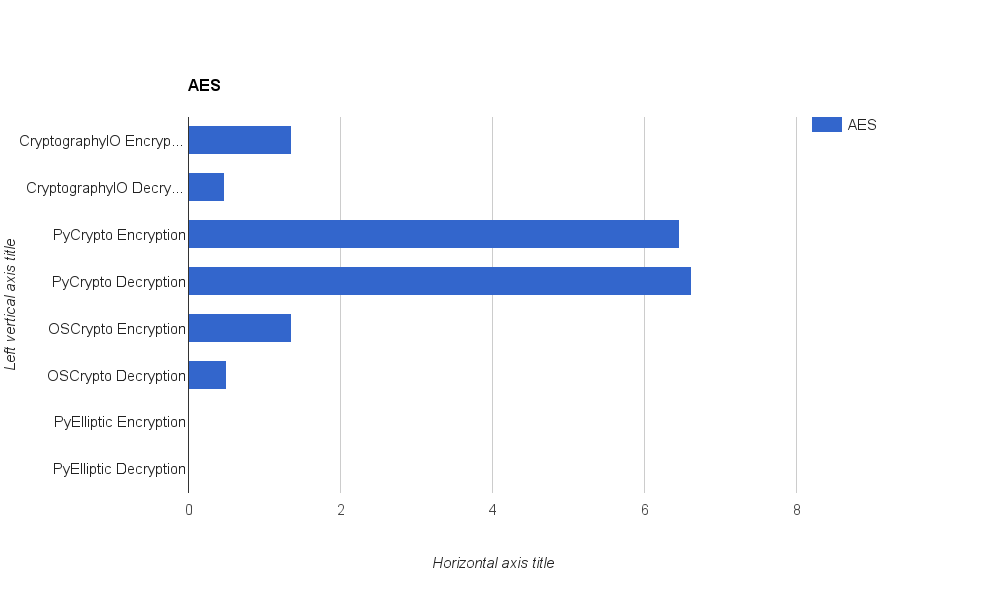
\includegraphics[width=0.7\linewidth]{./aes}
\caption{Average execution times for AES}
\label{fig:aes}
\end{figure}


\begin{figure}
\centering
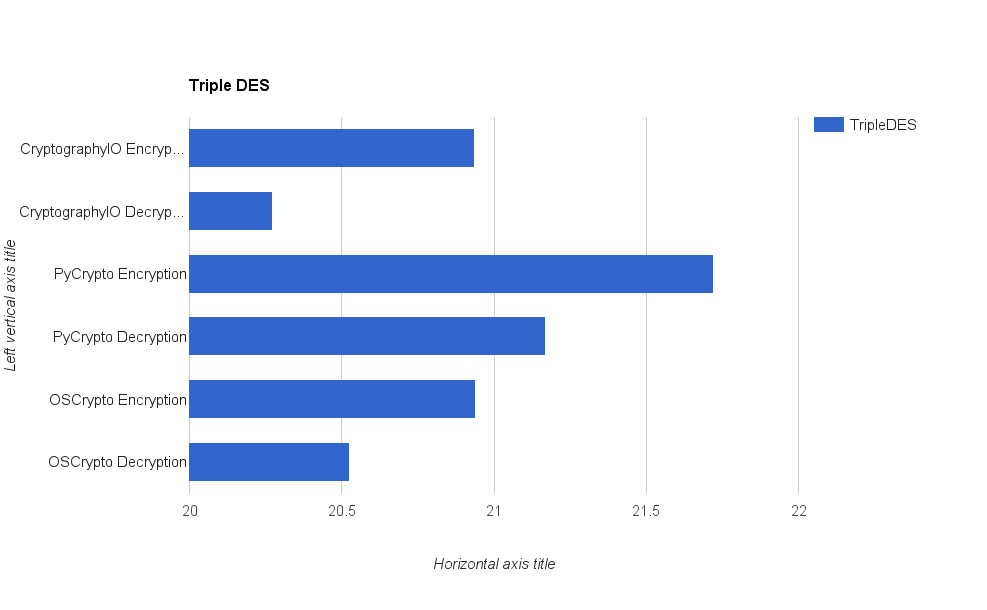
\includegraphics[width=0.7\linewidth]{./tripledes}
\caption{Average execution times for TripleDES}
\label{fig:tripledes}
\end{figure}



\begin{figure}
\centering
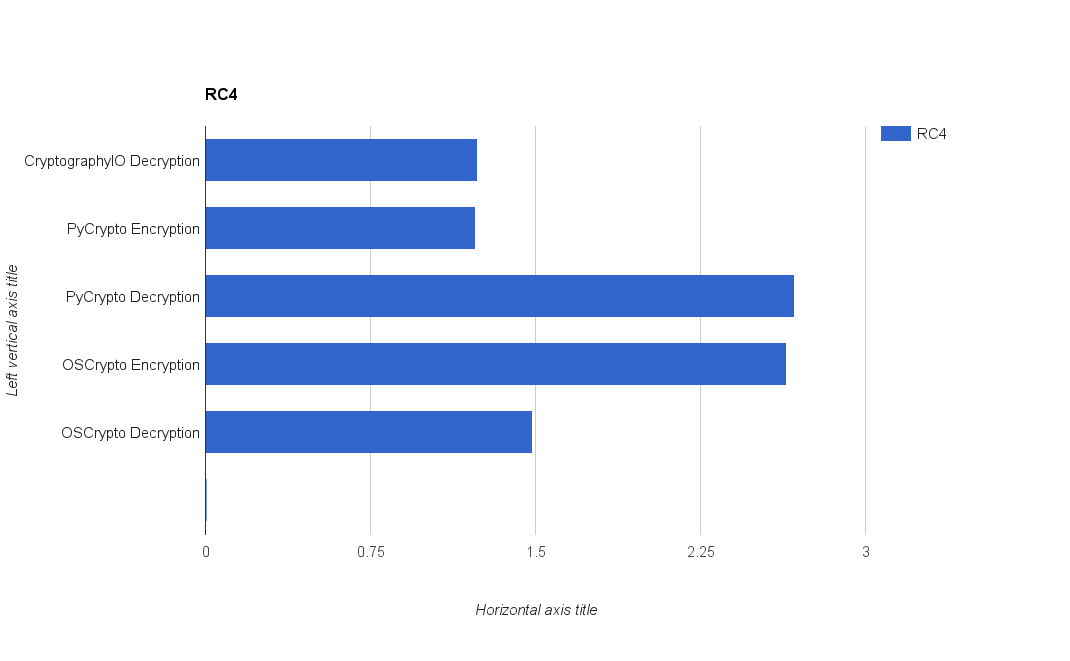
\includegraphics[width=0.7\linewidth]{./rc4}
\caption{Average execution times for RC4}
\label{fig:rc4}
\end{figure}

\subsection{Ease of Use}

Interms of ease of use OSCrpto was the easiest to approach for simple straight forward method calls, for example to encrypt with AES in CBC mode it was simply a matte of calling the \textit{aes\_cbc\_pkcs7\_encrypt} method and passing the key, plain text and the initialisation vector.

OSCrypto's simplicity becomes a problem when trying mix and match the various combinations of modes with each algorithm, this is completly unsupported. CryptographyIO is much better suited for this task.

CryptographyIO compensates for its increased verbosity by offering much greater flexibilty, immensely better documentation and intensely cool names for its packages such as \textit{cryptography.hazmat} for parts of the library which can potentially be hazardous when used incorrectly. The documentations is also quite detailed and well designed with the developers using Sphinx to generate beautiful documentation

PyCrypto is decent in terms of documenation with ancient java style docs. The docs is also missing a few methods but generally passable. Ease of use is similar to CryptographyIO but one might need to spend some extra time reading source code to understand the sometimes vague or missing sections of the documentation.

PyElliptic's documentation is a joke, its consists merely of a single page README file. Ease of use and flexibilty were passable but it was hard to confirm due it lack of widespread usage. 


\begin{figure}
\centering
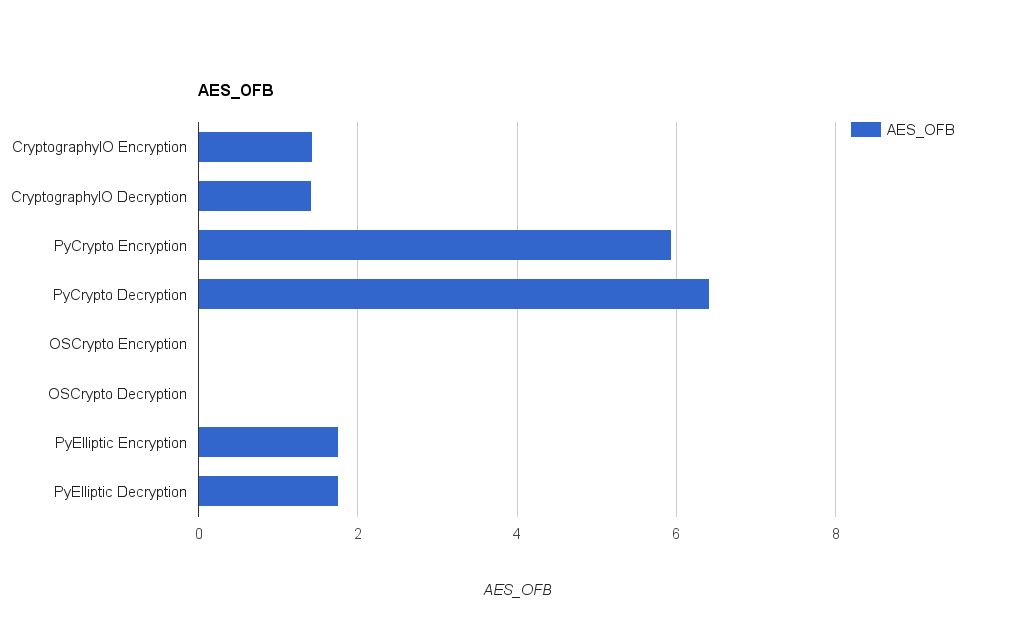
\includegraphics[width=0.7\linewidth]{./aesofb}
\caption{Average execution times for AES under OFB mode as a stream cipher}
\label{fig:aesofb}
\end{figure}

\begin{figure}
\centering
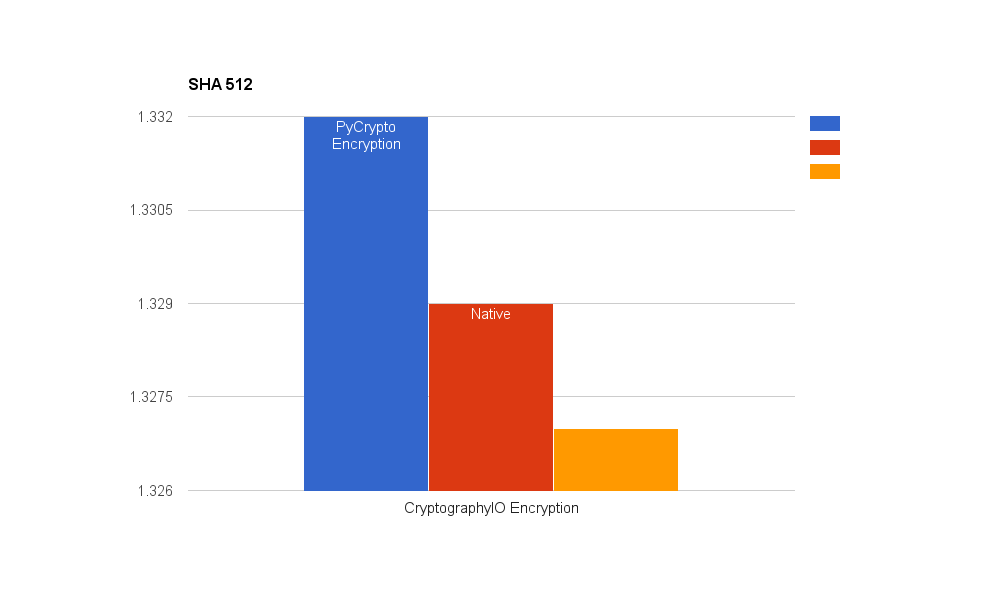
\includegraphics[width=0.7\linewidth]{./sha512}
\caption{Average execution times for SHA512}
\label{fig:sha512}
\end{figure}

\begin{figure}
\centering
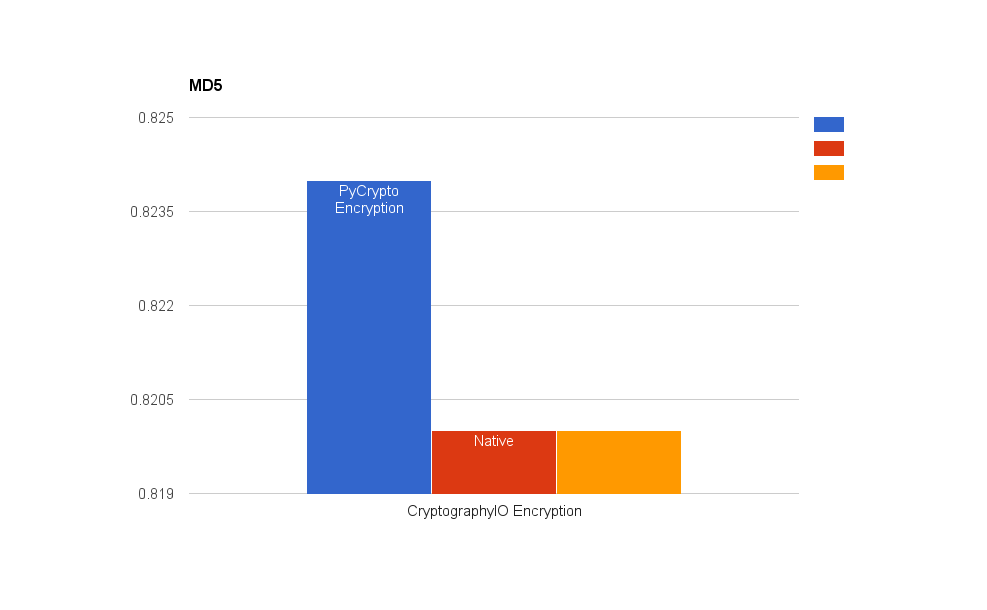
\includegraphics[width=0.7\linewidth]{./md5}
\caption{Average execution times for MD5}
\label{fig:md5}
\end{figure}

\section{SCP Benchmark}

The results of the SCP benchmark can be found in table \ref{table:resultsScp}. The test was copying a 5Mb file from my computer via a 30Mbps internet connection to uw1-320-02.uwb.edu. Almost all ciphers transferred the file in around 1.7 seconds. Stream ciphers such as ARC4 performed noticibly faster than a block cipher in CTR mode. Surprisingly TripleDes under CTR mode performed quite well while AES 256 took the longest time atleast initially.


\begin{figure}
\centering
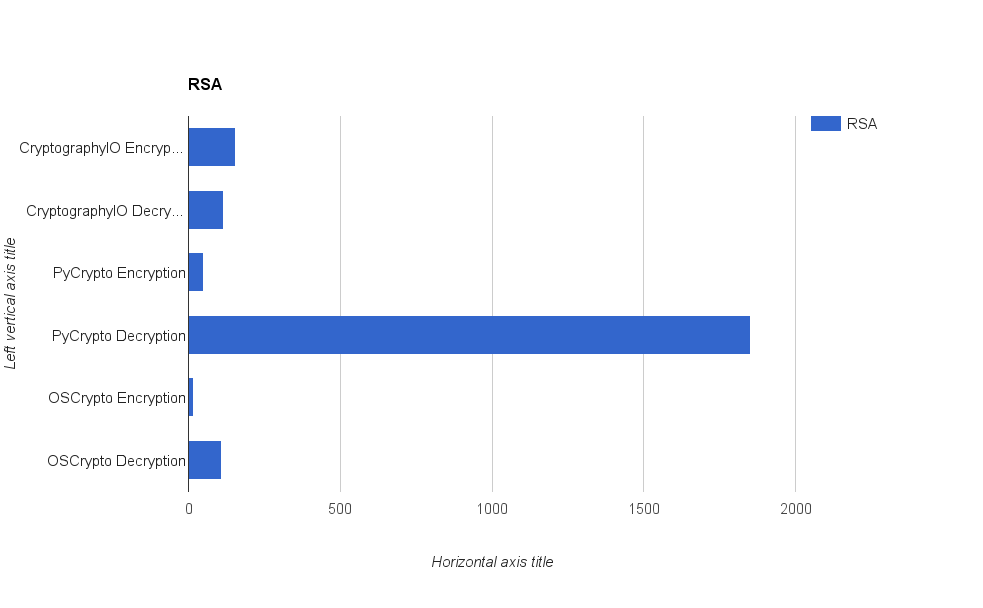
\includegraphics[width=0.7\linewidth]{./RSA}
\caption{Average execution times for RSA}
\label{fig:RSA}
\end{figure}

\begin{figure}
\centering
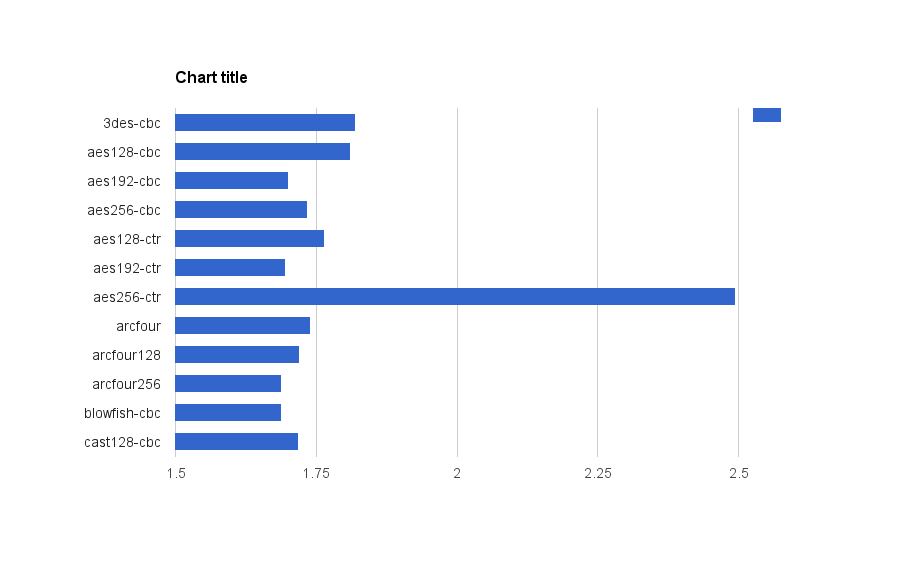
\includegraphics[width=0.7\linewidth]{./scpbench}
\caption{Average execution times when benchmarking SCP with various ciphers.}
\label{fig:scpbench}
\end{figure}



\section{Conclusion}

In conclusion Cryptography IO seems to be a well balanced library which is easy enough to use while still offering flexibilty and decent performance. In terms of secure hash functions, python's native haslib does a good enough job that no external library is needed. Pycrypto would be the next best option though its performance is abmysal. The developer seems to be actively developing pycrypto and it may improve in the future.








\begin{table}[]
\centering
\caption{Results of benchmarking tests}
\label{table:results1}
\begin{tabular}{|l|c|c|c|c|c|c|c|}
\hline
                          & AES\_OFB & AES   & RC4   & RSA      & TripleDES & SHA512 & MD5   \\ \hline
CryptographyIO Encryption & 1.433    & 1.355 & 1.237 & 154.291  & 20.936    & 1.332  & 0.824 \\ \hline
CryptographyIO Decryption & 1.418    & 0.473 & 1.226 & 114.577  & 20.274    &        &       \\ \hline
PyCrypto Encryption       & 5.945    & 6.463 & 2.677 & 49.177   & 21.72     & 1.329  & 0.82  \\ \hline
PyCrypto Decryption       & 6.416    & 6.615 & 2.64  & 1850.219 & 21.17     &        &       \\ \hline
OSCrypto Encryption       &          & 1.355 & 1.487 & 16.76    & 20.94     &        &       \\ \hline
OSCrypto Decryption       &          & 0.5   & 0.005 & 108.722  & 20.525    &        &       \\ \hline
PyElliptic Encryption     & 1.762    &       &       &          &           &        &       \\ \hline
PyElliptic Decryption     & 1.764    &       &       &          &           &        &       \\ \hline
Native                    &          &       &       &          &           & 1.327  & 0.82  \\ \hline
\end{tabular}
\end{table}

\begin{table}[]
\centering
\caption{SCP Benchmarking Results}
\label{table:resultsScp}
\begin{tabular}{|l|c|c|c|c|c|c|}
\hline
Algorithm    &      &      &      &      &      & Average \\ \hline
3des-cbc     & 1.92 & 1.73 & 1.72 & 2.02 & 1.71 & 1.82    \\ \hline
aes128-cbc   & 1.76 & 1.7  & 2.04 & 1.79 & 1.76 & 1.81    \\ \hline
aes192-cbc   & 1.69 & 1.7  & 1.71 & 1.68 & 1.72 & 1.7     \\ \hline
aes256-cbc   & 1.69 & 1.81 & 1.69 & 1.74 & 1.74 & 1.734   \\ \hline
aes128-ctr   & 1.93 & 1.69 & 1.76 & 1.71 & 1.73 & 1.764   \\ \hline
aes192-ctr   & 1.69 & 1.69 & 1.71 & 1.7  & 1.69 & 1.696   \\ \hline
aes256-ctr   & 5.54 & 1.73 & 1.7  & 1.78 & 1.72 & 2.494   \\ \hline
arcfour      & 1.98 & 1.67 & 1.69 & 1.68 & 1.68 & 1.74    \\ \hline
arcfour128   & 1.75 & 1.71 & 1.73 & 1.71 & 1.7  & 1.72    \\ \hline
arcfour256   & 1.67 & 1.68 & 1.69 & 1.71 & 1.69 & 1.688   \\ \hline
blowfish-cbc & 1.69 & 1.68 & 1.68 & 1.67 & 1.72 & 1.688   \\ \hline
cast128-cbc  & 1.69 & 1.75 & 1.73 & 1.73 & 1.69 & 1.718   \\ \hline
\end{tabular}
\end{table}



\end{document}

